\subsubsection{3D Vektorer}

[Beskrivelse af 3D Vektorer]


\subsubsection{Rotationsmatricer}
Hvis vi vil roterer et punkt eller en vektor omkring nul-punktet i et koordinatsystem kan vi bruge en rotationsmatrix\cite{rotationsmatricer}. En rotationsmatrix i 2D består af:
\begin{figure}[H]
  \centering
  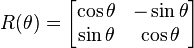
\includegraphics[width=5cm]{2D_vektor_rotationsmatrix.png}
  \caption{2D Rotationsmatricer. Taget fra https://en.wikipedia.org/wiki/Rotation\_matrix}
\end{figure}
Indsætter vi mængden af radianer vi vil dreje vores vektor og ganger dem sammen, ser vi at vektoren bliver drejet omkring nul-punktet med netop den mængde radianer. 
Hvis vi vil rotere en vektor/et punkt i 3D bliver det lidt mere komplekst. Vi vil så roterer 2 af punkterne i et plan omkring det sidste punkt, som dermed også virker som normalvektor til planet. Formlerne for at gøre dette er udviklet og frit tilgængelige på blandt andet Wikipedia's side om rotationsmatricer:
\begin{figure}[H]
  \centering
  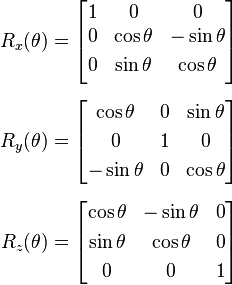
\includegraphics[width=5cm]{3D_vektor_rotationsmatrix.png}
  \caption{3D Rotationsmatricer. Taget fra https://en.wikipedia.org/wiki/Rotation\_matrix}
\end{figure}
Her skal vi, ligesom med 2D rotationsmatricer, bare indsætte vinklen og gange dem sammen med vektoren vi vil dreje.